\documentclass[12pt]{article}
\usepackage{parskip,amsmath,amssymb,enumerate,graphicx}
\usepackage[margin=.6in]{geometry}
\begin{document}
\subsection*{1}
\begin{enumerate}[a)]
    \item
        \begin{align*}
        f(n) &=
            \begin{cases}
            e^t, & \text{if }0 \leq t \leq 1 \\
            0, & \text{if }1 < t
            \end{cases}\\
            &= e^tu_{-1}(t) - e^tu_{-1}(t-1)\\
            F(s) &= \mathcal{L} \{e^tu_{-1}(t)\} - \mathcal{L}\{e^tu_{-1}(t-1)\}\\
                &= \frac{1}{s-1} - e\mathcal{L}\{e^{t-1}u_{-1}(t-1)\}\\
                &= \frac{1}{s-1} - e\frac{e^{-s}}{s-1} \\
                &= \frac{1-e^{1-s}}{s-1} \\
        \end{align*}
    \item
        \begin{align*}
            f(n) &=
                \begin{cases}
                t, & \text{if }0 \leq t \leq 1 \\
                0, & \text{if }1 < t
                \end{cases}\\
            &= tu_{-1}(t)-tu_{-1}(t-1)\\
            F(s) &= \mathcal{L}\{tu_{-1}(t)\} - \mathcal{L}\{tu_{-1}(t-1)\}\\
                &= \frac{1}{s^2} + \frac{d}{ds}\mathcal{L}\{u_{-1}(t-1)\}\\
                &= \frac{1}{s^2} + \frac{d}{ds}\frac{e^{-s}}{s} \\
                &= \frac{1}{s^2} - \frac{e^{-s}}{s} - \frac{e^{-s}}{s^2} \\
        \end{align*}
    \item
        \begin{align*}
            f(n) &=
                \begin{cases}
                t^2, & \text{if }0 \leq t \leq 3 \\
                0, & \text{if }3 < t
                \end{cases}\\
            &= t^2u_{-1}(t) - t^2u_{-1}(t-3)\\
            F(s) &= \mathcal{L} \{ t^2u_{-1}(t)\} - \mathcal{L}\{t^2u_{-1}(t-3)\}\\
                &=\frac{2}{s^3} + \frac{d}{ds} \bigg( -\frac{d}{ds} \mathcal{L}\{ u_{-1}(t-3)\} \bigg)\\
                &=\frac{2}{s^3} + \frac{d}{ds} \bigg( -\frac{d}{ds} \frac{e^{-3s}}{s} \bigg)\\
                &=\frac{2}{s^3} - \frac{d}{ds} \bigg( \frac{-3e^{-3s}}{s} - \frac{e^{-3s}}{s^2} \bigg)\\
                &=\frac{2}{s^3} + \frac{d}{ds} \bigg( \frac{-3e^{-3s}}{s} + \frac{e^{-3s}}{s^2} \bigg)\\
                &=\frac{2}{s^3} + \frac{-9e^{-3s}}{s} + \frac{-3e^{-3s}}{s^2} + \frac{-3e^{-3s}}{s^2} + \frac{-2e^{-3s}}{s^3}\\
                &= \frac{2-2e^{-3s} -6se^{-3s} - 9s^2e^{-3s}}{s^3}  \\
        \end{align*}
    \item
        \begin{align*}
            f(n) &=
                \begin{cases}
                \sin(4t), & \text{if }0 \leq t \leq \frac{\pi}{4} \\
                0, & \text{if }\frac{\pi}{4} < t
                \end{cases}\\
            &= \sin(4t)u_{-1}(t) - \sin(4t)u_{-1}(t- \frac{\pi}{4})\\
            F(s) &= \mathcal{L} \{\sin(4t)u_{-1}(t)\} - \mathcal{L} \{\sin(4t)u_{-1}(t- \frac{\pi}{4})\}\\
                &=\frac{4}{s^2 + 16} - \mathcal{L} \bigg \{  \frac{e^{4jt} - e^{-4jt}}{2j} u_{-1}(t- \frac{\pi}{4}) \bigg\}\\
                &=\frac{4}{s^2 + 16} - \frac{1}{2j} \bigg[\mathcal{L} \{ e^{4jt}u_{-1}(t- \frac{\pi}{4})\} - \mathcal{L} \{e^{-4jt} u_{-1}(t- \frac{\pi}{4}) \}\bigg]\\
                &=\frac{4}{s^2 + 16} - \frac{e^{\frac{\pi}{4}}}{2j} \bigg[\mathcal{L} \bigg\{ e^{4tj-\frac{\pi}{4}}u_{-1}(t- \frac{\pi}{4})\bigg\} - \mathcal{L} \bigg\{e^{-4jt-\frac{\pi}{4}} u_{-1}(t- \frac{\pi}{4}) \bigg\}\bigg]\\
                &=\frac{4}{s^2 + 16} - \frac{e^{\frac{\pi}{4}}}{2j} e^{-\frac{\pi}{4}s} \bigg[\mathcal{L} \bigg\{ e^{4tj}u_{-1}(t)\bigg\} - \mathcal{L} \bigg\{e^{-4jt} u_{-1}(t) \bigg\}\bigg]\\
                &=\frac{4}{s^2 + 16} - \frac{e^{\frac{\pi}{4}(1-s)}}{2j} \bigg[\frac{1}{s-4j} - \frac{1}{s+4j}\bigg]\\
                &=\frac{4}{s^2 + 16} - \frac{e^{\frac{\pi}{4}(1-s)}}{2j} \bigg[\frac{8j}{s^2+16}\bigg]\\
                &=\frac{4}{s^2 + 16} - e^{\frac{\pi}{4}(1-s)} \bigg[\frac{4}{s^2+16}\bigg]\\
                &=\frac{4 (1- e^{\frac{\pi}{4}(1-s)})}{s^2 + 16}\\
        \end{align*}
\end{enumerate}

\subsection*{2}
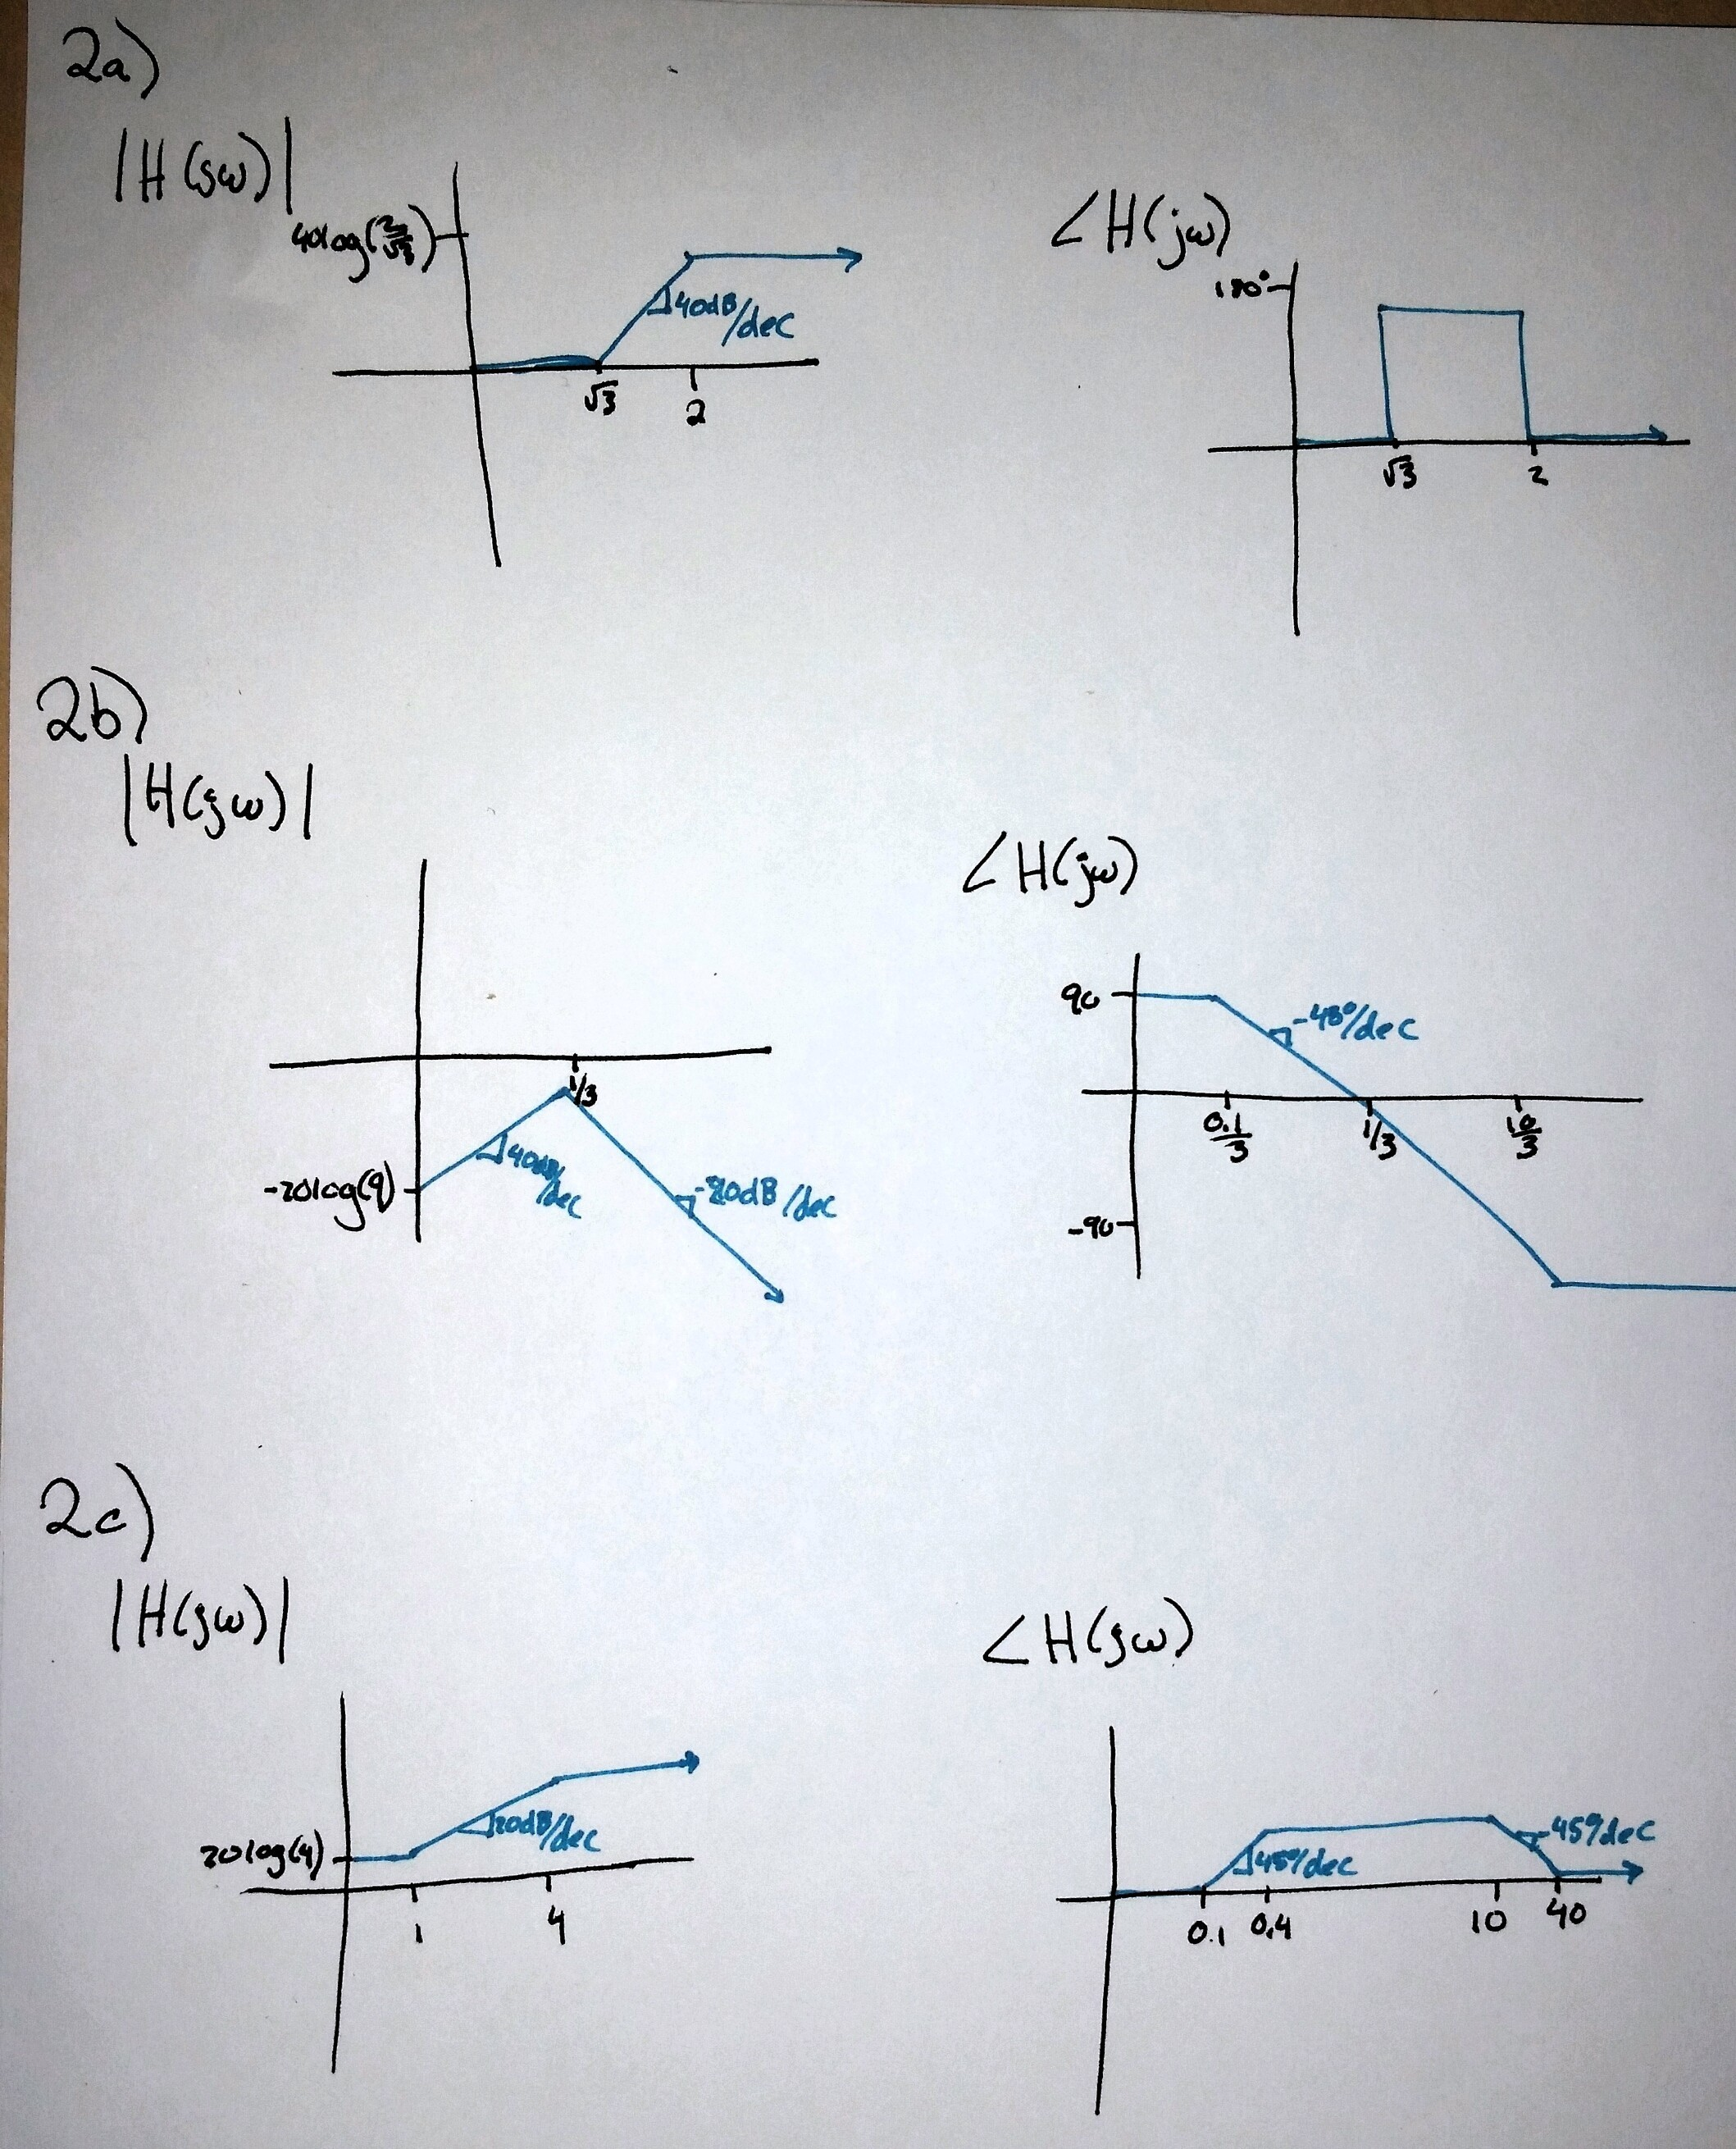
\includegraphics[width=15cm]{2.jpg}




\subsection*{3}
\begin{align*}
    G(s) & = \frac{s}{s^2 + 2s + 2}\\
    G(jw) &= \frac{jw}{-w^2 + 2jw + 2}\\
    G(j) &= \frac{j}{2j + 1} = \frac{1}{1-2j}\\
    |G(j)| &= \sqrt{1^2 + 2^2} = \sqrt{5}\\
    \angle G(j) &= 180 - \tan^{-1}(\frac{1}{2}) = 153\\
    G(jw) &= \frac{1}{\sqrt{5}e^{153j}}\\
\end{align*}
Steady state is achieved at $\frac{1}{\sqrt{5}e^{153j}} * e^{jwt}$


\subsection*{4}
\begin{enumerate}[a)]
    \item
    \begin{align*}
        Y(S) &= KC(S)P(S)U(S)\\
            & \implies U(S) = \frac{Y(S)}{KC(S)P(S)}\\
        U(S) &= R(S) - KC(S)P(S)U(S)\\
        \frac{Y(S)}{KC(S)P(S)} &= R(S) - KC(S)P(S) \frac{Y(S)}{KC(S)P(S)}\\
        Y(S) &= KC(S)P(S)[R(S) - Y(S)]\\
        Y(S)[]+KC(S)P(S)] &= KC(S)P(S)R(S)\\
        \frac{Y(S)}{R(S)} &= \frac{KC(S)P(S)}{} + KC(S)P(S)
    \end{align*}
    \item The magnitude graph ends on a downward slope so the function must have more poles than zeros which means that the degree of the denominator is greater than that of the numerator, so C(S)P(S) must be a proper rational. Since H(S) contains the same power of C(S)P(S) in its numerator and denominator and no other S's its properness will match that of C(S)P(S) meaning that H(S) is also a proper rational.
\end{enumerate}

















\end{document}
